
%% bare_conf.tex
%% V1.4b
%% 2015/08/26
%% by Michael Shell
%% See:
%% http://www.michaelshell.org/
%% for current contact information.
%%
%% This is a skeleton file demonstrating the use of IEEEtran.cls
%% (requires IEEEtran.cls version 1.8b or later) with an IEEE
%% conference paper.
%%
%% Support sites:
%% http://www.michaelshell.org/tex/ieeetran/
%% http://www.ctan.org/pkg/ieeetran
%% and
%% http://www.ieee.org/

%%*************************************************************************
%% Legal Notice:
%% This code is offered as-is without any warranty either expressed or
%% implied; without even the implied warranty of MERCHANTABILITY or
%% FITNESS FOR A PARTICULAR PURPOSE! 
%% User assumes all risk.
%% In no event shall the IEEE or any contributor to this code be liable for
%% any damages or losses, including, but not limited to, incidental,
%% consequential, or any other damages, resulting from the use or misuse
%% of any information contained here.
%%
%% All comments are the opinions of their respective authors and are not
%% necessarily endorsed by the IEEE.
%%
%% This work is distributed under the LaTeX Project Public License (LPPL)
%% ( http://www.latex-project.org/ ) version 1.3, and may be freely used,
%% distributed and modified. A copy of the LPPL, version 1.3, is included
%% in the base LaTeX documentation of all distributions of LaTeX released
%% 2003/12/01 or later.
%% Retain all contribution notices and credits.
%% ** Modified files should be clearly indicated as such, including  **
%% ** renaming them and changing author support contact information. **
%%*************************************************************************


% *** Authors should verify (and, if needed, correct) their LaTeX system  ***
% *** with the testflow diagnostic prior to trusting their LaTeX platform ***
% *** with production work. The IEEE's font choices and paper sizes can   ***
% *** trigger bugs that do not appear when using other class files.       ***                          ***
% The testflow support page is at:
% http://www.michaelshell.org/tex/testflow/



\documentclass[conference]{IEEEtran}
% Some Computer Society conferences also require the compsoc mode option,
% but others use the standard conference format.
%
% If IEEEtran.cls has not been installed into the LaTeX system files,
% manually specify the path to it like:
% \documentclass[conference]{../sty/IEEEtran}





% Some very useful LaTeX packages include:
% (uncomment the ones you want to load)


% *** MISC UTILITY PACKAGES ***
%
%\usepackage{ifpdf}
% Heiko Oberdiek's ifpdf.sty is very useful if you need conditional
% compilation based on whether the output is pdf or dvi.
% usage:
% \ifpdf
%   % pdf code
% \else
%   % dvi code
% \fi
% The latest version of ifpdf.sty can be obtained from:
% http://www.ctan.org/pkg/ifpdf
% Also, note that IEEEtran.cls V1.7 and later provides a builtin
% \ifCLASSINFOpdf conditional that works the same way.
% When switching from latex to pdflatex and vice-versa, the compiler may
% have to be run twice to clear warning/error messages.






% *** CITATION PACKAGES ***
%
%\usepackage{cite}
% cite.sty was written by Donald Arseneau
% V1.6 and later of IEEEtran pre-defines the format of the cite.sty package
% \cite{} output to follow that of the IEEE. Loading the cite package will
% result in citation numbers being automatically sorted and properly
% "compressed/ranged". e.g., [1], [9], [2], [7], [5], [6] without using
% cite.sty will become [1], [2], [5]--[7], [9] using cite.sty. cite.sty's
% \cite will automatically add leading space, if needed. Use cite.sty's
% noadjust option (cite.sty V3.8 and later) if you want to turn this off
% such as if a citation ever needs to be enclosed in parenthesis.
% cite.sty is already installed on most LaTeX systems. Be sure and use
% version 5.0 (2009-03-20) and later if using hyperref.sty.
% The latest version can be obtained at:
% http://www.ctan.org/pkg/cite
% The documentation is contained in the cite.sty file itself.






% *** GRAPHICS RELATED PACKAGES ***
%
\ifCLASSINFOpdf
  % \usepackage[pdftex]{graphicx}
  % declare the path(s) where your graphic files are
  % \graphicspath{{../pdf/}{../jpeg/}}
  % and their extensions so you won't have to specify these with
  % every instance of \includegraphics
  % \DeclareGraphicsExtensions{.pdf,.jpeg,.png}
\else
  % or other class option (dvipsone, dvipdf, if not using dvips). graphicx
  % will default to the driver specified in the system graphics.cfg if no
  % driver is specified.
  % \usepackage[dvips]{graphicx}
  % declare the path(s) where your graphic files are
  % \graphicspath{{../eps/}}
  % and their extensions so you won't have to specify these with
  % every instance of \includegraphics
  % \DeclareGraphicsExtensions{.eps}
\fi
% graphicx was written by David Carlisle and Sebastian Rahtz. It is
% required if you want graphics, photos, etc. graphicx.sty is already
% installed on most LaTeX systems. The latest version and documentation
% can be obtained at: 
% http://www.ctan.org/pkg/graphicx
% Another good source of documentation is "Using Imported Graphics in
% LaTeX2e" by Keith Reckdahl which can be found at:
% http://www.ctan.org/pkg/epslatex
%
% latex, and pdflatex in dvi mode, support graphics in encapsulated
% postscript (.eps) format. pdflatex in pdf mode supports graphics
% in .pdf, .jpeg, .png and .mps (metapost) formats. Users should ensure
% that all non-photo figures use a vector format (.eps, .pdf, .mps) and
% not a bitmapped formats (.jpeg, .png). The IEEE frowns on bitmapped formats
% which can result in "jaggedy"/blurry rendering of lines and letters as
% well as large increases in file sizes.
%
% You can find documentation about the pdfTeX application at:
% http://www.tug.org/applications/pdftex





% *** MATH PACKAGES ***
%
%\usepackage{amsmath}
% A popular package from the American Mathematical Society that provides
% many useful and powerful commands for dealing with mathematics.
%
% Note that the amsmath package sets \interdisplaylinepenalty to 10000
% thus preventing page breaks from occurring within multiline equations. Use:
%\interdisplaylinepenalty=2500
% after loading amsmath to restore such page breaks as IEEEtran.cls normally
% does. amsmath.sty is already installed on most LaTeX systems. The latest
% version and documentation can be obtained at:
% http://www.ctan.org/pkg/amsmath





% *** SPECIALIZED LIST PACKAGES ***
%
%\usepackage{algorithmic}
% algorithmic.sty was written by Peter Williams and Rogerio Brito.
% This package provides an algorithmic environment fo describing algorithms.
% You can use the algorithmic environment in-text or within a figure
% environment to provide for a floating algorithm. Do NOT use the algorithm
% floating environment provided by algorithm.sty (by the same authors) or
% algorithm2e.sty (by Christophe Fiorio) as the IEEE does not use dedicated
% algorithm float types and packages that provide these will not provide
% correct IEEE style captions. The latest version and documentation of
% algorithmic.sty can be obtained at:
% http://www.ctan.org/pkg/algorithms
% Also of interest may be the (relatively newer and more customizable)
% algorithmicx.sty package by Szasz Janos:
% http://www.ctan.org/pkg/algorithmicx




% *** ALIGNMENT PACKAGES ***
%
%\usepackage{array}
% Frank Mittelbach's and David Carlisle's array.sty patches and improves
% the standard LaTeX2e array and tabular environments to provide better
% appearance and additional user controls. As the default LaTeX2e table
% generation code is lacking to the point of almost being broken with
% respect to the quality of the end results, all users are strongly
% advised to use an enhanced (at the very least that provided by array.sty)
% set of table tools. array.sty is already installed on most systems. The
% latest version and documentation can be obtained at:
% http://www.ctan.org/pkg/array


% IEEEtran contains the IEEEeqnarray family of commands that can be used to
% generate multiline equations as well as matrices, tables, etc., of high
% quality.




% *** SUBFIGURE PACKAGES ***
%\ifCLASSOPTIONcompsoc
%  \usepackage[caption=false,font=normalsize,labelfont=sf,textfont=sf]{subfig}
%\else
%  \usepackage[caption=false,font=footnotesize]{subfig}
%\fi
% subfig.sty, written by Steven Douglas Cochran, is the modern replacement
% for subfigure.sty, the latter of which is no longer maintained and is
% incompatible with some LaTeX packages including fixltx2e. However,
% subfig.sty requires and automatically loads Axel Sommerfeldt's caption.sty
% which will override IEEEtran.cls' handling of captions and this will result
% in non-IEEE style figure/table captions. To prevent this problem, be sure
% and invoke subfig.sty's "caption=false" package option (available since
% subfig.sty version 1.3, 2005/06/28) as this is will preserve IEEEtran.cls
% handling of captions.
% Note that the Computer Society format requires a larger sans serif font
% than the serif footnote size font used in traditional IEEE formatting
% and thus the need to invoke different subfig.sty package options depending
% on whether compsoc mode has been enabled.
%
% The latest version and documentation of subfig.sty can be obtained at:
% http://www.ctan.org/pkg/subfig




% *** FLOAT PACKAGES ***
%
%\usepackage{fixltx2e}
% fixltx2e, the successor to the earlier fix2col.sty, was written by
% Frank Mittelbach and David Carlisle. This package corrects a few problems
% in the LaTeX2e kernel, the most notable of which is that in current
% LaTeX2e releases, the ordering of single and double column floats is not
% guaranteed to be preserved. Thus, an unpatched LaTeX2e can allow a
% single column figure to be placed prior to an earlier double column
% figure.
% Be aware that LaTeX2e kernels dated 2015 and later have fixltx2e.sty's
% corrections already built into the system in which case a warning will
% be issued if an attempt is made to load fixltx2e.sty as it is no longer
% needed.
% The latest version and documentation can be found at:
% http://www.ctan.org/pkg/fixltx2e


%\usepackage{stfloats}
% stfloats.sty was written by Sigitas Tolusis. This package gives LaTeX2e
% the ability to do double column floats at the bottom of the page as well
% as the top. (e.g., "\begin{figure*}[!b]" is not normally possible in
% LaTeX2e). It also provides a command:
%\fnbelowfloat
% to enable the placement of footnotes below bottom floats (the standard
% LaTeX2e kernel puts them above bottom floats). This is an invasive package
% which rewrites many portions of the LaTeX2e float routines. It may not work
% with other packages that modify the LaTeX2e float routines. The latest
% version and documentation can be obtained at:
% http://www.ctan.org/pkg/stfloats
% Do not use the stfloats baselinefloat ability as the IEEE does not allow
% \baselineskip to stretch. Authors submitting work to the IEEE should note
% that the IEEE rarely uses double column equations and that authors should try
% to avoid such use. Do not be tempted to use the cuted.sty or midfloat.sty
% packages (also by Sigitas Tolusis) as the IEEE does not format its papers in
% such ways.
% Do not attempt to use stfloats with fixltx2e as they are incompatible.
% Instead, use Morten Hogholm'a dblfloatfix which combines the features
% of both fixltx2e and stfloats:
%
% \usepackage{dblfloatfix}
% The latest version can be found at:
% http://www.ctan.org/pkg/dblfloatfix




% *** PDF, URL AND HYPERLINK PACKAGES ***
%
%\usepackage{url}
% url.sty was written by Donald Arseneau. It provides better support for
% handling and breaking URLs. url.sty is already installed on most LaTeX
% systems. The latest version and documentation can be obtained at:
% http://www.ctan.org/pkg/url
% Basically, \url{my_url_here}.




% *** Do not adjust lengths that control margins, column widths, etc. ***
% *** Do not use packages that alter fonts (such as pslatex).         ***
% There should be no need to do such things with IEEEtran.cls V1.6 and later.
% (Unless specifically asked to do so by the journal or conference you plan
% to submit to, of course. )


% correct bad hyphenation here
\hyphenation{op-tical net-works semi-conduc-tor}

\usepackage{amssymb}
\setcounter{tocdepth}{3}
\usepackage{graphicx}
\usepackage{mathtools}
\DeclarePairedDelimiter\ceil{\lceil}{\rceil}
\DeclarePairedDelimiter\floor{\lfloor}{\rfloor}

\usepackage{url}

\begin{document}
%
% paper title
% Titles are generally capitalized except for words such as a, an, and, as,
% at, but, by, for, in, nor, of, on, or, the, to and up, which are usually
% not capitalized unless they are the first or last word of the title.
% Linebreaks \\ can be used within to get better formatting as desired.
% Do not put math or special symbols in the title.
\title{Characterizing Performance and Power towards Efficient Synchronization of GPU Kernels}


% author names and affiliations
% use a multiple column layout for up to three different
% affiliations
\author{\IEEEauthorblockN{Islam Harb}
\IEEEauthorblockA{Department of Computer Science\\
Virginia Tech \\
Blacksburg, Virginia, USA\\
Electronic Research Institute, Egypt \\
iharb@vt.edu}
\and
\IEEEauthorblockN{Wu-Chun Feng}
\IEEEauthorblockA{Department of Computer Science \\
	Department of Electrical and Computer Engineering \\
	Virginia Tech\\
	Blacksburg, Virginia, USA\\
	wfeng@vt.edu}}

% conference papers do not typically use \thanks and this command
% is locked out in conference mode. If really needed, such as for
% the acknowledgment of grants, issue a \IEEEoverridecommandlockouts
% after \documentclass

% for over three affiliations, or if they all won't fit within the width
% of the page, use this alternative format:
% 
%\author{\IEEEauthorblockN{Michael Shell\IEEEauthorrefmark{1},
%Homer Simpson\IEEEauthorrefmark{2},
%James Kirk\IEEEauthorrefmark{3}, 
%Montgomery Scott\IEEEauthorrefmark{3} and
%Eldon Tyrell\IEEEauthorrefmark{4}}
%\IEEEauthorblockA{\IEEEauthorrefmark{1}School of Electrical and Computer Engineering\\
%Georgia Institute of Technology,
%Atlanta, Georgia 30332--0250\\ Email: see http://www.michaelshell.org/contact.html}
%\IEEEauthorblockA{\IEEEauthorrefmark{2}Twentieth Century Fox, Springfield, USA\\
%Email: homer@thesimpsons.com}
%\IEEEauthorblockA{\IEEEauthorrefmark{3}Starfleet Academy, San Francisco, California 96678-2391\\
%Telephone: (800) 555--1212, Fax: (888) 555--1212}
%\IEEEauthorblockA{\IEEEauthorrefmark{4}Tyrell Inc., 123 Replicant Street, Los Angeles, California 90210--4321}}




% use for special paper notices
%\IEEEspecialpapernotice{(Invited Paper)}




% make the title area
\maketitle

% As a general rule, do not put math, special symbols or citations
% in the abstract

\begin{abstract}
	There is a lack of support for explicit synchronization in GPUs between the streaming multiprocessors (SMs) adversely impacts the performance of the GPUs to efficiently perform inter-block communication. In this paper, we present several approaches to inter-block synchronization using explicit/implicit CPU-based and dynamic parallelism (DP) mechanisms. Although this topic has been addressed in previous research studies, there has been neither a solid quantification of such overhead, nor guidance on when to use each of the different approaches. Therefore, we quantify the synchronization overhead relative to the number of kernel launches and the input data sizes. The quantification, in turn, provides insight as to \emph{when} to use each of the aforementioned synchronization mechanisms in a target application. Our results show that implicit CPU synchronization has a significant overhead that hurts the application performance when using medium to large data sizes with relatively large number of kernel launches (i.e. \url{~}1100-5000). Hence, it is recommended to use explicit CPU synchronization with these configurations. In addition, among the three different approaches, we conclude that dynamic parallelism (DP) is the most efficient with small data sizes (i.e., $\leq$128k bytes), regardless of the number of kernel launches. Also, Dynamic Parallelism (DP), implicitly, performs inter-block (i.e. global) synchronization with no CPU intervention. Therefore,  DP significantly reduces the power consumed by the CPU and PCIe for global synchronization. Our findings show that DP reduces the power consumption by \url{~}8-10\%. However, DP-based synchronization is a trade-off, in which it is accompanied by \url{~}2-5\% performance loss.
	
	%	\keywords{GPU, CPU Synchronization, Dynamic Parallelism}
\end{abstract}


\begin{IEEEkeywords} GPU, CPU Synchronization, Dynamic Parallelism \end{IEEEkeywords}

% For peer review papers, you can put extra information on the cover
% page as needed:
% \ifCLASSOPTIONpeerreview
% \begin{center} \bfseries EDICS Category: 3-BBND \end{center}
% \fi
%
% For peerreview papers, this IEEEtran command inserts a page break and
% creates the second title. It will be ignored for other modes.
\IEEEpeerreviewmaketitle

\section{Introduction}
\label{sec:intro}

To address the lack of direct support for native inter-block synchronization on the GPU,
%primitives, 
researchers have adopted indirect mechanisms such as GPU barrier synchronization~\cite{proc9}, implicit CPU barrier synchronization, explicit CPU barrier synchronization, and more recently, dynamic parallelism (DP). However, these mechanisms incur non-trivial overhead compared to a hypothetical native synchronization primitive implemented in hardware.

Synchronization within a GPU can be classified into intra-block and inter-block synchronization. Intra-block synchronization coordinates the threads \emph{within} a streaming multiprocessor (SM) in the context of shared on-chip memory.
%indicates the data communication between threads on the level of the shared on-chip memory. That means the communication happens on the same streaming multiprocessor (SM). 
On the other hand, inter-block synchronization coordinates data communication between threads that span \emph{across} different streaming multiprocessors (SMs) in the context of global off-chip memory. Off-chip (i.e., global) memory access latency is significantly higher than that of the on-chip (i.e., local) memory. Therefore, inter-block synchronization incurs orders of magnitude higher overhead than 
%is way slower than 
that of the intra-block synchronization. In this study, we focus on inter-block communication/global barrier synchronization, which is also referred to as inter-streaming-multiprocessor (i.e., inter-SM) synchronization.  

Traditionally, global synchronization is done via terminating the current kernel execution, then re-launching it again or even launching another kernel. By default, the CUDA kernel launches are asynchronous. That means the CPU will offload the computation to the GPU and return immediately, as shown in Figure~\ref{fig:cpu_sync}(a). We refer to this mechanism as \emph{implicit} CPU global synchronization. On the other hand, NVIDIA provides a mechanism to support synchronous (i.e. blocking) kernel launches by calling ``cudaDeviceSynchronize()" API after the kernel launch. This API blocks at the CPU until the GPU finishes the current kernel computation, as shown in Figure~\ref{fig:cpu_sync}(b). We refer to this mechanism as \emph{explicit} CPU global synchronization. For this, the latter incurs larger overhead. However, under specific circumstances, our study shows that the \emph{implicit CPU global synchronization} may experience a significant performance degradation, thus the use of \emph{explicit CPU global synchronization} is required.
%In this study, we show that implicit barrier synchronization has its downsides that make it breaks in some scenarios, and hence the explicit way is more convenient. On the other hand, 

Recently, an indirect method for GPU-based synchronization, namely \emph{Dynamic Parallelism (DP)}~\cite{proc5,proc5_}, has been introduced in recent NVIDIA architectures (e.g. GK110), in an attempt to lessen the CPU-GPU communication overhead and enhance the dynamic load balancing as shown in ~\cite{proc1,proc2,proc3,proc6}. DP represents implicit On-GPU global barrier synchronization without CPU intervention. However, much of the recent work that has been done with DP indicates that it incurs significant overhead~\cite{proc1,proc3,proc4,proc7,proc8}, thus it is claimed to be \emph{impractical}. On the other hand, several researches~\cite{free_launch, DTBL} took place to introduce alternatives to the Dynamic Parallelism because of its high overhead. Our analysis uncovers scenarios where DP outperforms the other synchronization mechanisms. 

The explicit GPU global synchronization~\cite{proc9} might be competitive with DP. However, NVIDIA introduces ``\_\_threadfence()" API to, theoretically, ensure correctness of inter-block communication. The overhead of the \emph{explicit GPU synchronization} with the ``\_\_threadfence()" is significantly high~\cite{proc12}. In addition, it comes with a limitation on the number of blocks executing on the GPU, in which it should \emph{not} exceed the number of the Streaming Multiprocessors (SMs). As such, explicit GPU global synchronization is opted to be out of scope of this paper.
%The explicit GPU-based global barrier synchronization~\cite{proc9}eliminates the overhead of CPU kernel launch, however, its need to the "\_\_theadfence()" incurs a significant overhead. In addition, it has a limitation on the number of blocks executing on the GPU, which is platform-dependent.

%Each of the synchronization approaches has its weakness, as well as its strength points. 
Previous work in GPU kernel launch and synchronization has not provided guidance on when it is appropriate to use each of the aforementioned approaches to synchronization within a specific target application.
Although some work has been done to characterize the overhead of synchronization primitives and protocols, it has been mainly from the hardware (i.e., platform) point of view. In addition, dynamic parallelism (DP) is missing from these previous studies. 

Therefore, in this paper, we conduct a comprehensive study and characterization of the overhead for the different approaches to synchronization for the GPU.
%CPU and GPU global barrier synchronization mechanisms. 
Our contributions are as follows. 
\begin{itemize}
	\item
	Guidelines to choose the most appropriate synchronization mechanism based on application's parameters.
	\item
	Quantification of the kernel launch time and the synchronization overhead for each of the mechanisms vs. the number of kernel launches and the data sizes. 
	\item
	We are the first to use the Dynamic Parallelism as a mean of global synchronization. In addition, We show its power consumption advantage compared to the other mechanisms (i.e.,CPU-based global synchronization). 
	\item
	Realization of synthetic micro-kernel and application benchmarks to stress-test the different approaches to synchronization. 
\end{itemize}

The rest of the paper is organized as follows. Section~\ref{sec:RW} presents the work related to synchronization and dynamic parallelism (DP). Section~\ref{sec:approach_app} discusses the applications and its role in studying the overhead of the synchronization mechanisms. Section~\ref{sec:eval}, then, analyzes and quantifies this overhead of each synchronization mechanism. In addition, we conduct a comparison of performance vs. power consumption for both the DP-based and the other synchronization mechanisms. Finally, section~\ref{sec:conclusion} concludes our work and discusses future work.

%\begin{table}
%	\caption{Specification of K20c Compute Capabilities}
%	\begin{center}
%		\renewcommand{\arraystretch}{1.4}
%		\setlength\tabcolsep{3pt}
%		\begin{tabular}{llll}
%			\hline\noalign{\smallskip}
%			Feature & sm\_20 & sm\_30 & sm\_35\\
%			\noalign{\smallskip}
%			\hline
%			\noalign{\smallskip}
%			Max Threads per SM & 1536 & 2048 & 2048 \\
%			Max Co-operative Thread Array (CTAs) per SM & 8 & 16 & 16  \\
%			Shared Memory Capacity per SM & 48 & 48 & 48  \\
%			Register File (RF) Capacity per SM & 128 KB & 256 KB & 256 KB  \\
%			Max Registers per Thread & 63 & 63 & 255  \\
%			Number of Registers Per Block & 32K & 64K & 64K  \\
%			\hline
%		\end{tabular}
%	\end{center}
%	\label{tab:kepler1}
%\end{table}

\begin{figure}
	%\vspace{2cm}
	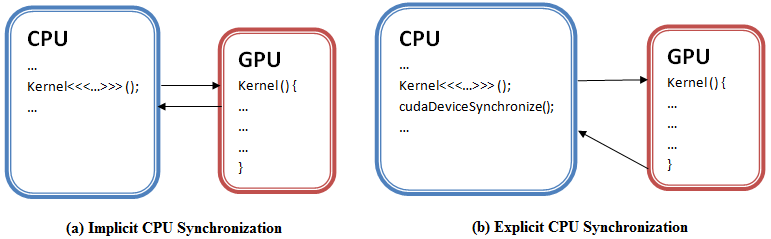
\includegraphics[width=1.0\columnwidth, height=2.5cm]{cpu_sync.png}
	\caption{The CPU Synchronization Mechanisms}
	\label{fig:cpu_sync}
\end{figure}

\section{Related Work}
\label{sec:RW}
Our work is related to the area of synchronization protocols for many-core architectures and characterization of the Dynamic Parallelism. 

The explicit GPU-based synchronization can be realized by either lock-based or lock-free techniques as introduced in~\cite{proc9}. Both techniques require the number of blocks to be less than or equal to the number of the streaming multiprocessors in the GPU to avoid the potential deadlock. Their study shows that the explicit GPU-based synchronization may incur a significant overhead, relative to the implicit CPU synchronization, when using the memory fence API.  Mehmet et al.~\cite{proc10} have used the wavefront parallelism to mitigate the explicit GPU-based synchronization overhead. Meanwhile, Gupta et al.~\cite{proc13} have introduced the persistent thread concept to overcome the limitations on the number of blocks in the explicit GPU-based synchronization mechanism. However, none of these work considered the Dynamic Parallelism.

The work of David et al.~\cite{proc11} focus on the synchronization over multiple layers with the emphasis on the cache-coherency and locks. Stuart et al. ~\cite{proc16} conducted a research on the efficient synchronization primitives (e.g. atomic accesses) over many-core architectures. However, the their work is on characterizing the synchronization overhead based on many-core architecture and hardware targets. Both don't consider the applications configurations and parameters. In addition, the former study is meant for the CPU but it cannot be directly mapped to the GPU environment. 

On the other hand, several efforts has been introduced to reduce or eliminate the global barrier synchronizations~\cite{proc14,proc15,proc17}. These are optimization studies to lessen the synchronization points within an application. They didn't provide any characterization of the overhead of the synchronization mechanisms.  

Jin et al.~\cite{proc4} lead a study for characterizing the dynamically-formed parallelism on irregular (i.e. unstructured) applications on GPUs. They conclude that the Dynamic Parallelism causes \url{~}1.21x slowdown due to its non-trivial overhead. Dimarco et al.~\cite{proc3} carried out a study on the use of the Dynamic Parallelism to accelerate clustering algorithms, which also confirms its significant overhead. However, both works are addressing DP for dynamic load balancing in irregularity in applications. It didn't discuss synchronization overhead. In addition, they didn't cover structured or regular applications. Our analysis provides DP overhead quantification and guidelines on when to use each of the global barrier synchronization, including the Dynamic Parallelism, for each target application.  

%Springer provides you with a complete integrated \LaTeX{} document class
%(\texttt{llncs.cls}) for multi-author books such as those in the LNCS
%series. Papers not complying with the LNCS style will be reformatted.
%This can lead to an increase in the overall number of pages. We would
%therefore urge you not to squash your paper.
%
%Please always cancel any superfluous definitions that are
%not actually used in your text. If you do not, these may conflict with
%the definitions of the macro package, causing changes in the structure
%of the text and leading to numerous mistakes in the proofs.
%
%If you wonder what \LaTeX{} is and where it can be obtained, see the
%``\textit{LaTeX project site}'' (\url{http://www.latex-project.org})
%and especially the webpage ``\textit{How to get it}''
%(\url{http://www.latex-project.org/ftp.html}) respectively.
%
%When you use \LaTeX\ together with our document class file,
%\texttt{llncs.cls},
%your text is typeset automatically in Computer Modern Roman (CM) fonts.
%Please do
%\emph{not} change the preset fonts. If you have to use fonts other
%than the preset fonts, kindly submit these with your files.
%
%Please use the commands \verb+\label+ and \verb+\ref+ for
%cross-references and the commands \verb+\bibitem+ and \verb+\cite+ for
%references to the bibliography, to enable us to create hyperlinks at
%these places.
%
%For preparing your figures electronically and integrating them into
%your source file we recommend using the standard \LaTeX{} \verb+graphics+ or
%\verb+graphicx+ package. These provide the \verb+\includegraphics+ command.
%In general, please refrain from using the \verb+\special+ command.
%
%Remember to submit any further style files and
%fonts you have used together with your source files.
%
%\subsubsection{Headings.}
%
%Headings should be capitalized
%(i.e., nouns, verbs, and all other words
%except articles, prepositions, and conjunctions should be set with an
%initial capital) and should,
%with the exception of the title, be aligned to the left.
%Words joined by a hyphen are subject to a special rule. If the first
%word can stand alone, the second word should be capitalized.
%
%Here are some examples of headings: ``Criteria to Disprove
%Context-Freeness of Collage Language", ``On Correcting the Intrusion of
%Tracing Non-deterministic Programs by Software", ``A User-Friendly and
%Extendable Data Distribution System", ``Multi-flip Networks:
%Parallelizing GenSAT", ``Self-determinations of Man".
%
%\subsubsection{Lemmas, Propositions, and Theorems.}
%
%The numbers accorded to lemmas, propositions, and theorems, etc. should
%appear in consecutive order, starting with Lemma 1, and not, for
%example, with Lemma 11.
%
%\subsection{Figures}
%
%For \LaTeX\ users, we recommend using the \emph{graphics} or \emph{graphicx}
%package and the \verb+\includegraphics+ command.
%
%Please check that the lines in line drawings are not
%interrupted and are of a constant width. Grids and details within the
%figures must be clearly legible and may not be written one on top of
%the other. Line drawings should have a resolution of at least 800 dpi
%(preferably 1200 dpi). The lettering in figures should have a height of
%2~mm (10-point type). Figures should be numbered and should have a
%caption which should always be positioned \emph{under} the figures, in
%contrast to the caption belonging to a table, which should always appear
%\emph{above} the table; this is simply achieved as matter of sequence in
%your source.
%
%Please center the figures or your tabular material by using the \verb+\centering+
%declaration. Short captions are centered by default between the margins
%and typeset in 9-point type (Fig.~\ref{fig:example} shows an example).
%The distance between text and figure is preset to be about 8~mm, the
%distance between figure and caption about 6~mm.
%
%To ensure that the reproduction of your illustrations is of a reasonable
%quality, we advise against the use of shading. The contrast should be as
%pronounced as possible.
%
%If screenshots are necessary, please make sure that you are happy with
%the print quality before you send the files.
%%\begin{figure}
%%\centering
%%\includegraphics[height=6.2cm]{eijkel2}
%%\caption{One kernel at $x_s$ (\emph{dotted kernel}) or two kernels at
%%$x_i$ and $x_j$ (\textit{left and right}) lead to the same summed estimate
%%at $x_s$. This shows a figure consisting of different types of
%%lines. Elements of the figure described in the caption should be set in
%%italics, in parentheses, as shown in this sample caption.}
%%\label{fig:example}
%%\end{figure}
%
%Please define figures (and tables) as floating objects. Please avoid
%using optional location parameters like ``\verb+[h]+" for ``here".
%
%\paragraph{Remark 1.}
%
%In the printed volumes, illustrations are generally black and white
%(halftones), and only in exceptional cases, and if the author is
%prepared to cover the extra cost for color reproduction, are colored
%pictures accepted. Colored pictures are welcome in the electronic
%version free of charge. If you send colored figures that are to be
%printed in black and white, please make sure that they really are
%legible in black and white. Some colors as well as the contrast of
%converted colors show up very poorly when printed in black and white.
%
%\subsection{Formulas}
%
%Displayed equations or formulas are centered and set on a separate
%line (with an extra line or halfline space above and below). Displayed
%expressions should be numbered for reference. The numbers should be
%consecutive within each section or within the contribution,
%with numbers enclosed in parentheses and set on the right margin --
%which is the default if you use the \emph{equation} environment, e.g.,
%\begin{equation}
%  \psi (u) = \int_{o}^{T} \left[\frac{1}{2}
%  \left(\Lambda_{o}^{-1} u,u\right) + N^{\ast} (-u)\right] dt \;  .
%\end{equation}
%
%Equations should be punctuated in the same way as ordinary
%text but with a small space before the end punctuation mark.
%
%\subsection{Footnotes}
%
%The superscript numeral used to refer to a footnote appears in the text
%either directly after the word to be discussed or -- in relation to a
%phrase or a sentence -- following the punctuation sign (comma,
%semicolon, or period). Footnotes should appear at the bottom of
%the
%normal text area, with a line of about 2~cm set
%immediately above them.\footnote{The footnote numeral is set flush left
%and the text follows with the usual word spacing.}
%
%\subsection{Program Code}
%
%Program listings or program commands in the text are normally set in
%typewriter font, e.g., CMTT10 or Courier.
%
%\medskip
%
%\noindent
%{\it Example of a Computer Program}
%\begin{verbatim}
%program Inflation (Output)
%  {Assuming annual inflation rates of 7%, 8%, and 10%,...
%   years};
%   const
%     MaxYears = 10;
%   var
%     Year: 0..MaxYears;
%     Factor1, Factor2, Factor3: Real;
%   begin
%     Year := 0;
%     Factor1 := 1.0; Factor2 := 1.0; Factor3 := 1.0;
%     WriteLn('Year  7% 8% 10%'); WriteLn;
%     repeat
%       Year := Year + 1;
%       Factor1 := Factor1 * 1.07;
%       Factor2 := Factor2 * 1.08;
%       Factor3 := Factor3 * 1.10;
%       WriteLn(Year:5,Factor1:7:3,Factor2:7:3,Factor3:7:3)
%     until Year = MaxYears
%end.
%\end{verbatim}
%%
%\noindent
%{\small (Example from Jensen K., Wirth N. (1991) Pascal user manual and
%report. Springer, New York)}
%
%\subsection{Citations}
%
%For citations in the text please use
%square brackets and consecutive numbers: \cite{jour}, \cite{lncschap},
%\cite{proceeding1} -- provided automatically
%by \LaTeX 's \verb|\cite| \dots\verb|\bibitem| mechanism.
%
%\subsection{Page Numbering and Running Heads}
%
%There is no need to include page numbers. If your paper title is too
%long to serve as a running head, it will be shortened. Your suggestion
%as to how to shorten it would be most welcome.

%\begin{figure}
%	%\vspace{2.5cm}
%	\includegraphics[width=1.0\columnwidth, height=9cm]{LDC_Overview.png}
%	\caption{A Flow Chart for the Lid-Drive Cavity Application}
%	\label{fig:ldc_overview}
%\end{figure}


\section{Approach and Applications}
\label{sec:approach_app}
We implement a synthetic micro-benchmark to analyze and understand the behavior of the CPU and GPU (i.e. Dynamic Parallelism) synchronization mechanisms over a variety spectrum of workloads.  The micro-benchmark represents computations with different memory access characteristics. The kernels (i.e. computations) that require low to no read/write global memory access are classified as light-weight kernels. On the other hand the kernels that require average to intense read/write global memory accesses are classified as average-to-heavy-weight kernels. Our micro-benchmark includes kernels with memory access patterns as follows.  
\begin{itemize}
	\item
	Empty Kernel.
	\item
	Shared-Memory Kernel: Computations read/write from/to shared memory only.
	\item
	Global Memory Kernel: Computations read/write from/to global memory. Allocation is done by either the CPU or the GPU.
	\item
	Local Memory Kernel: Computations read/write from/to private memory or registers only.
	\item
	Others: combination of the above primitives. 
\end{itemize}

Apart from the micro-bench mark, we have selected two applications for more insights and evaluation. They are a good approximation of real-world applications.  

\begin{itemize}
	\item
	\textbf{The Lid-Driven Cavity (LDC)}: A computational fluid dynamic application that has stress, viscosity and pressure calculations on a mesh of a \emph{default} size 3x4096x4096. Each mesh cell is a double-precision floating point that occupies 8 bytes~\cite{cfd_blk_size}.
	\item
	\textbf{The Heat2D}: NVIDIA open source heat transfer simulation in a two-dimensional space~\cite{heat_code}. 
\end{itemize}

\section{Experiments Discussion and Evaluation}
\label{sec:eval}
For each of the experiments, we did 20 runs and then took the average to make our results resilient to the external uncontrolled errors. 

In order to quantify the synchronization overhead, we examine each of the synchronization mechanisms versus the number of kernel launches and the input data sizes (i.e. mesh sizes). The data type, in all applications, is double-precision floating point (i.e., 8 bytes). That means, mesh size can be translated into \emph{``bytes"} unit via multiplying the dimensions by ``8". For instance, mesh size of 128x128 is equivalent to 128x128x8 = 128 KBytes (KB). In addition, the mesh size affects directly on the number of blocks running on the GPU. Thus, it relates to the number of synchronization points and its overhead. The block size is fixed to 16x8 threads. Therefore, alternatively, the mesh size can be translated to the number of blocks which can be calculated as shown in \ref{blk_eqn}. For instance, data mesh size of 128x128 is equivalent to 128 Blocks.

\small
\begin{equation} 
\label{blk_eqn}
	Blocks = \ceil*{\frac{Mesh\_Dim\_X}{16}} * \ceil*{\frac{Mesh\_Dim\_Y}{8}} 
\end{equation}
\normalsize

We implement the applications with the three different synchronization mechanisms: the implicit CPU, the explicit CPU and the Dynamic Parallelism. We evaluate their power consumption, performance and overhead on both Kepler K20c and Tesla K20Xm GPUs with CUDA 6.0. The computational kernel is kept the same across all the variants. The explicit CPU synchronization mechanism requires the addition of  ``cudaDeviceSynchronize()" at the host side only. As for the Dynamic Parallelism, we implemented an auxiliary kernel that is launched once from the CPU side, and then it will manage all the launches and synchronization of the computational kernel within the GPU.  

We used \emph{NVIDIA Profiler} to collect numbers and analysis reports. It reports a breakdown that shows the kernel launch time (i.e. Overhead) and the execution time (i.e. Computation time) separately for the CPU synchronization mechanisms. However, with Dynamic Parallelism, it reports an integrated number for both launch and execution times . Since the computational kernel is untouched, the execution time should remain the same across all the synchronization mechanisms. Thus, we subtract the execution time, of the CPU synchronization run, from the integrated number reported in the DP run, to obtain the overall synchronization overhead (i.e. launch and sync).

\begin{figure}
	%\vspace{5cm}
	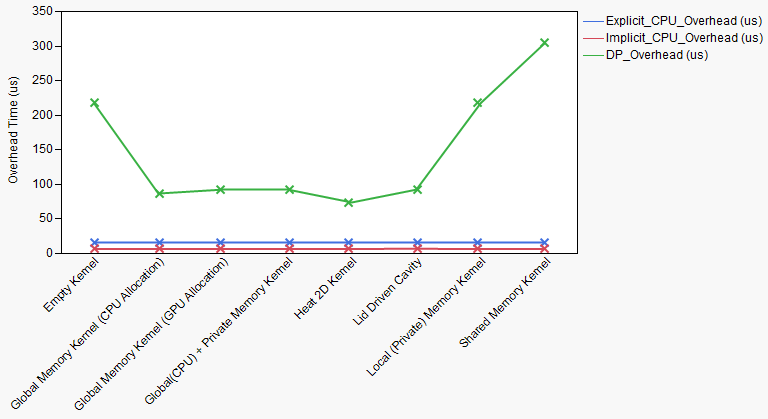
\includegraphics[width=1.0\columnwidth, height=5cm]{charaterize_overhead_arcoss_apps.png}
	\caption{The Synchronization Overhead Across Multiple Workloads}
	\label{fig:cpu_dp}
\end{figure}

The implicit CPU synchronization mechanism is recognized for its best performance and its least overhead among the aforementioned synchronization mechanisms. Therefore, we use it to characterize and classify our benchmark as shown in Figure~\ref{fig:cpu_dp}. It shows the overhead of the three mechanisms with 1000 kernel launches and 4096x4096 mesh size each. The number of kernel launches (i.e., 1000) is recommended by the domain scientists for the LDC. The implicit CPU synchronization outperforms both the explicit CPU synchronization and the Dynamic Parallelism, which is already expected. It is worth to mention that the Dynamic Parallelism has significantly larger overhead with light-weight kernels (e.g. empty, local or shared memory computations) than that of the medium-to-heavy-weight kernels (e.g. global memory computations, LDC and Heat2D). 

In the next subsections, we pick representatives of each of the light-weight and medium-to-heavy-weight kernels for further analysis. The ``Empty" and the ``Shared-Memory" Kernels represent the former category. Meanwhile, the ``Lid-Driven Cavity" and the ``Heat2D" Kernels represent the latter category. 

\subsection{Light-Weight Kernels}
We examined the synchronization overhead versus the number of kernel launches (i.e. 1-10k) for the light-weight kernels. Figure~\ref{fig:empty} and ~\ref{fig:shared} show the synchronization overhead for the ``Empty" Kernel and the ``Shared-Memory" kernel respectively. This experiment answers the research question on which synchronization mechanism is appropriate for the light-weight kernels, given the number of kernel launches. It shows the cut-off (i.e. \url{~5k} launches), at which the Dynamic Parallelism and the Explicit CPU synchronization outperform the Implicit CPU synchronization. This is due to the fact that the implicit CPU synchronization is a non-blocking mechanism. That means, it allows multiple kernel launches from the CPU side, even if it can't be all served and hence queued. So at a certain limit, it has to do a time consuming flush for the accumulated tasks in the queues. This limit is at 5k kernel launches with the light-weight kernels. 

\begin{figure}
	%\vspace{0.5cm}
	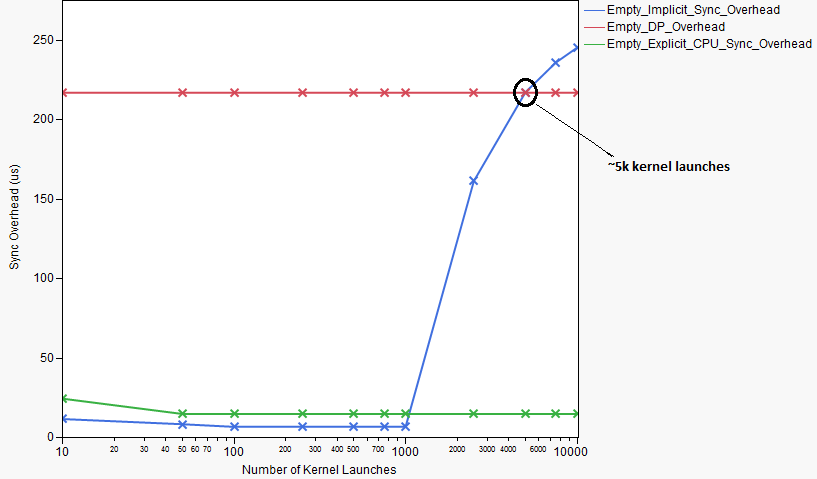
\includegraphics[width=1.0\columnwidth, height=5cm]{empty_kernel_sync_log_1.png}
	\caption{The Synchronization Overhead vs. No. of Kernel Launches -- Empty Kernel}
	\label{fig:empty}
\end{figure}
\begin{figure}
	%\vspace{5cm}
	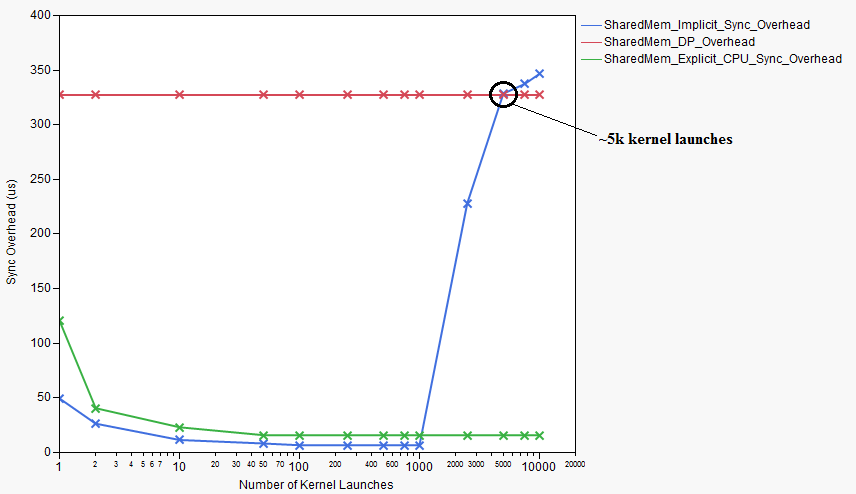
\includegraphics[width=1.0\columnwidth, height=5cm]{shared_mem_kernel_log.png}
	\caption{The Synchronization Overhead vs. No. of Kernel Launches -- Shared-Memory Kernel}
	\label{fig:shared}
\end{figure}

\subsection{Medium-to-Heavy-Weight Kernels}
Similarly, we examined the synchronization overhead versus the number of kernel launches (i.e. 1-10k) for the medium-to-heavy-weight kernels. Figure~\ref{fig:heat} and ~\ref{fig:ldc} show the synchronization overhead for the ``Heat2D" and the ``LDC" Kernels. In this case, we aim to answer the research question on which synchronization mechanism is appropriate for the medium-to-heavy-weight kernels, given the number of kernel launches. It shows the cut-off (i.e. 1100 launches), at which the Dynamic Parallelism and the Explicit CPU synchronization outperform the Implicit CPU synchronization. This is due to the same reason of queues flushing.

\begin{figure}
	%\vspace{5cm}
	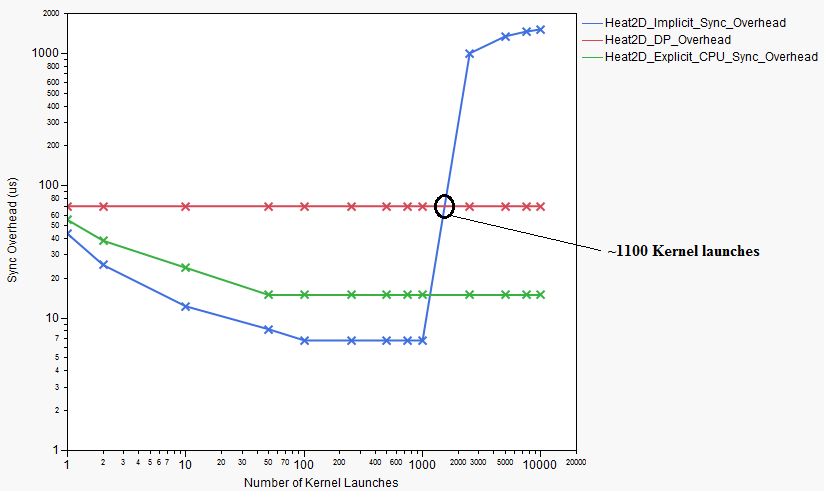
\includegraphics[width=1.0\columnwidth, height=5cm]{heat2d_sync_log.png}
	\caption{The Synchronization Overhead vs. No. of Kernel Launches -- Heat2D Kernel}
	\label{fig:heat}
\end{figure}
\begin{figure}
	%\vspace{2.5cm}
	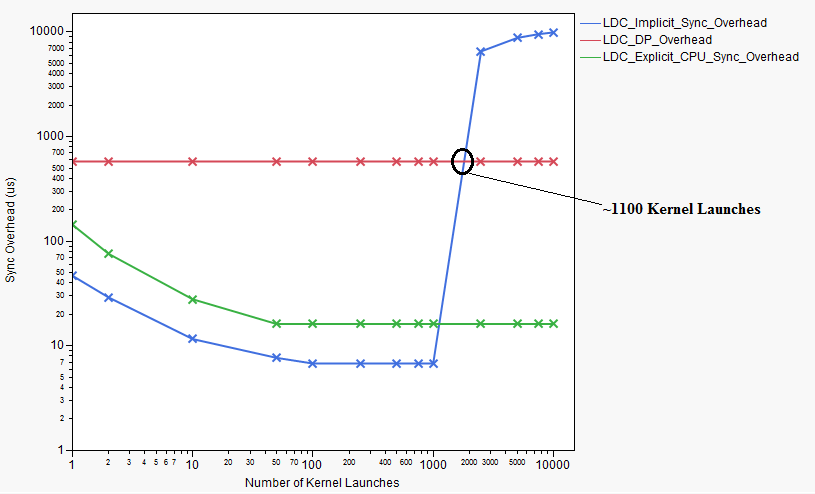
\includegraphics[width=1.0\columnwidth, height=5cm]{ldc_sync_log.png}
	\caption{The Synchronization Overhead vs. No. of Kernel Launches -- LDC Kernel}
	\label{fig:ldc}
\end{figure}

\subsection{Synchronization Overhead vs. Data Size}
The data size is an effective factor in determining the number of blocks that are executing on the GPU. We believe that the synchronization overhead increases with the increase of the data size. Therefore, we need to answer the research question about the data size cut-off at which the \emph{implicit CPU synchronization mechanism} remains robust (i.e. No performance degradation) given the previous cut-offs of the number of kernel launches. Figure~\ref{fig:implicit_vs_data_size} shows that the data size should be $\leq$ 128x128 (128 KB), in order to achieve high performance with large number of kernel launches (i.e. $\geq$ 1000).
 
\begin{figure}
	%\vspace{2.5cm}
	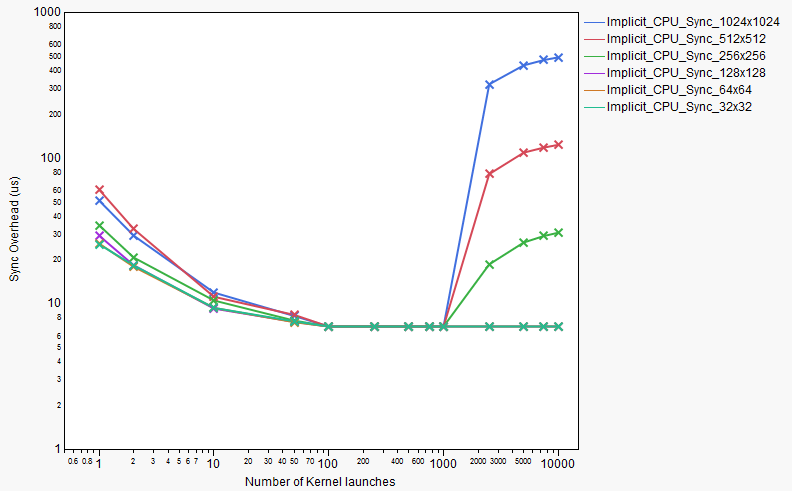
\includegraphics[width=1.0\columnwidth, height=5cm]{All_data_sizes_vs_number_kernel_launch.png}
	\caption{The Implicit CPU Synchronization Overhead vs. Data Size -- LDC Kernel}
	\label{fig:implicit_vs_data_size}
\end{figure}

On the other hand, we evaluate the overhead of the implicit CPU vs. the explicit CPU vs. the Dynamic Parallelism synchronization mechanism across the different data sizes. Figure~\ref{fig:sync_vs_data_size} shows that the overhead of dynamic parallelism is the least among the three synchronization mechanisms, when the data size is small (i.e. $<=$ 128x128 or 128 KB) regardless of the number of kernel launches. Therefore, the Dynamic Parallelism is the most appropriate synchronization mechanism for applications of relatively small input data sizes. This conclusion is confirmed and clarified in figure~\ref{fig:sync_vs_data_size_64x64}, that shows the synchronization overhead with the Lid-Driven Cavity (LDC) of 32 KB data size .

\begin{figure}
	%\vspace{5cm}
	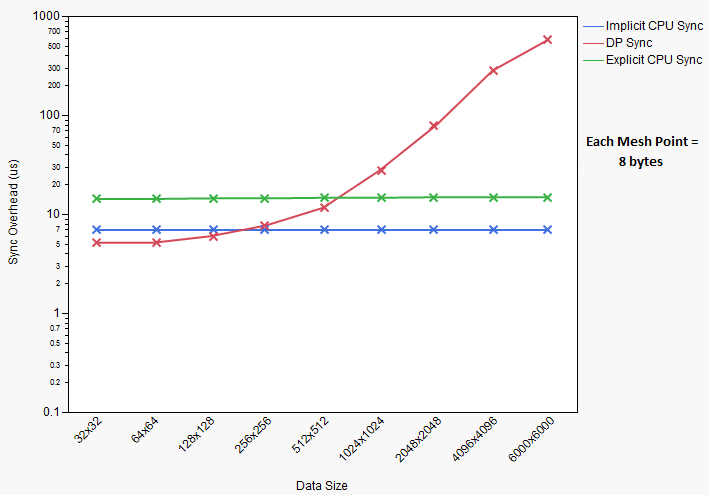
\includegraphics[width=1.0\columnwidth, height=5cm]{data_size_vs_sync_overhead.png}
	\caption{The Synchronization Overhead vs. Data Size -- LDC Kernel}
	\label{fig:sync_vs_data_size}
\end{figure}
\begin{figure}
	%\vspace{5cm}
	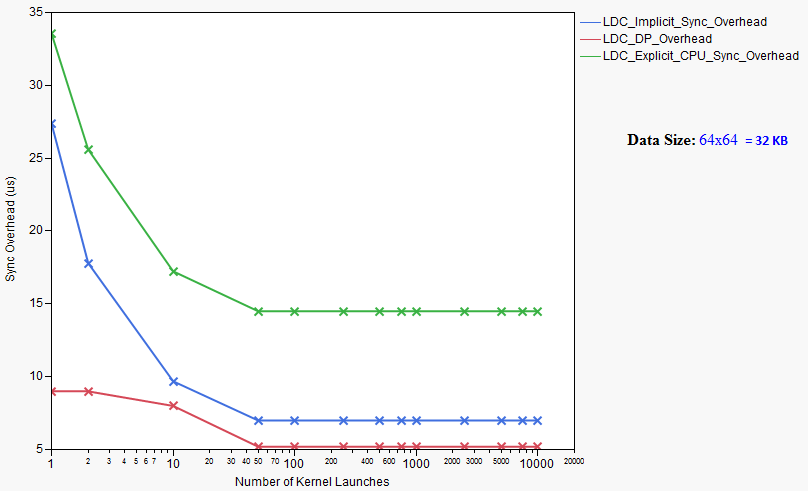
\includegraphics[width=1.0\columnwidth, height=5cm]{ldc_sync_log_64x64.png}
	\caption{The Synchronization Overhead vs. 64x64 Data Size -- LDC Kernel}
	\label{fig:sync_vs_data_size_64x64}
\end{figure}


%Table~\ref{tab:ldc_k20c}
%\begin{table}[th!]
%	\scriptsize
%	\caption{Power Consumption and Performance For LDC on Tesla K20c}
%	\centering
%	\begin{tabular}{c|c|c}
%		\hline
%		\bfseries  & \bfseries \begin{tabular}{c}
%			GPU-Based \\
%			Sync \\ 
%		\end{tabular}  & \bfseries \begin{tabular}{c}
%		CPU-Based \\
%		Sync \\ 
%	\end{tabular} \\
%	\hline\hline
%	Power Consumption & \url{~142 Watts} & \url{~153 Watts} \\
%	\hline
%	Execution Time & \url{~25.2 Sec} & \url{~24.7 Sec} \\
%	\hline
%\end{tabular}
%\label{tab:ldc_k20c}
%\end{table}

\begin{figure}
	%\vspace{5cm}
	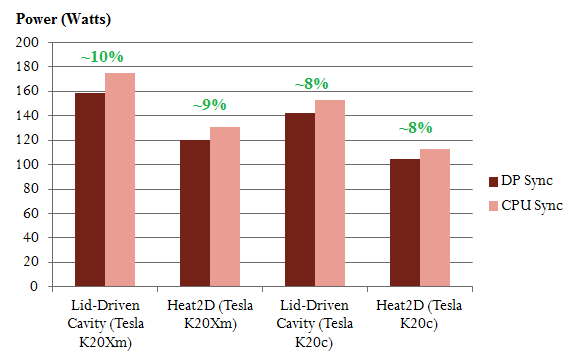
\includegraphics[width=1.0\columnwidth, height=4cm]{Pow_readings.png}
	\caption{DP vs. CPU: Power Consumption of the LDC and Heat2D Over Tesla K20c and Tesla K20Xm}
	\label{fig:pow}
\end{figure}

\begin{figure}
	%\vspace{5cm}
	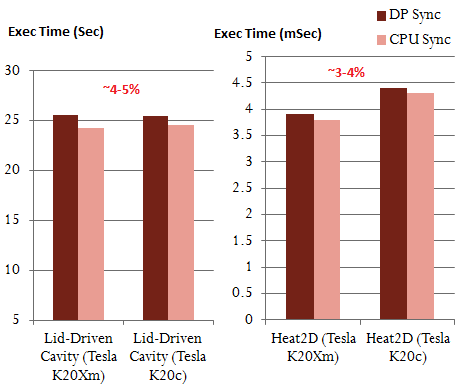
\includegraphics[width=1.0\columnwidth, height=4cm]{Perf_readings_1.png}
	\caption{DP vs. CPU: Execution Time of the LDC and Heat2D Over Tesla K20c and Tesla K20Xm}
	\label{fig:perf}
\end{figure}

\subsection{Power vs. Performance Trade-Off}

Unlike CPU-based global synchronization, DP globally synchronize the kernel running on the GPU without CPU intervention. Hence, Dynamic Parallelism reduces the power significantly by cutting the portions consumed by the CPU and the PCIe. We are concerned since power/energy saving is critical towards the exascale computing realization. 

We used the \emph{NVIDIA Management Library} (NVML) to collect power readings using ``nvmlDeviceGetPowerUsage()" API. The power reading is sampled during the execution lifetime and then averaged out. The sample count is \url{~25-30}.

In this section, implicit CPU-based and the DP-based global synchronizations have been compared with respect to the power and performance (i.e. execution time). we exclude the synthetic micro-benchmarks as numbers/readings will not be realistic with respect to the power consumption. Therefore, we report only the LDC and the Heat2D benchmarks. Our experiments are performed over both Tesla K20c and K20Xm platforms. Figure~\ref{fig:pow} shows the power consumption of the LDC and the Heat2D for both the \emph{implicit CPU-based} and the \emph{Dynamic Parallelism GPU-based} global synchronization mechanisms. DP global synchronization reduced the power consumption significantly by \url{~8-10}\% and \url{~8-9}\% for both the LDC and the Heat2D respectively. However, this power consumption improvement has a trade-off, in which there is a slight performance degradation accompanied with the DP mechanism compared to the CPU-based mechanism. Figure~\ref{fig:perf} shows that the DP global synchronization slightly increases the execution time by \url{~4-5}\% and \url{~2-3}\% for both the LDC and the Heat2D respectively.  

%Table~\ref{tab:heat2D_k20c}
%\begin{table}[th!]
%	\scriptsize
%	\caption{Power Consumption and Performance For Heat2D on Tesla K20c}
%	\centering
%	\begin{tabular}{c|c|c}
%		\hline
%		\bfseries  & \bfseries \begin{tabular}{c}
%			GPU-Based \\
%			Sync \\ 
%		\end{tabular}  & \bfseries \begin{tabular}{c}
%		CPU-Based \\
%		Sync \\ 
%	\end{tabular} \\
%	\hline\hline
%	Power Consumption & \url{~105 Watts} & \url{~113 Watts} \\
%	\hline
%	Execution Time & \url{~4.4 mSec} & \url{~4.2 mSec} \\
%	\hline
%\end{tabular}
%\label{tab:heat2D_k20c}
%\end{table}


\section{Conclusion and Future Work}
\label{sec:conclusion}
There is no explicit support for the Inter-Block synchronization. Several global synchronization mechanisms and protocols have been introduced during the past couple of years. However, there is still neither solid quantification nor comprehensive characterization for the overhead of the different synchronization mechanisms. Hence, we carried out a study to characterize the overhead of the known synchronization mechanisms. Our goal is to answer research questions about when and for which application, a specific synchronization mechanism should be used. We covered the implicit CPU synchronization, the explicit CPU synchronization and the Dynamic Parallelism in this study. Meanwhile, we are looking into extending our work by including the explicit GPU-based synchronization~\cite{proc9} with the \emph{Persistent Thread}~\cite{proc13} approach . 

Our results have challenged the idea that the \emph{implicit CPU synchronization} mechanism always has the best performance and the least overhead. With the large number of kernel launches, the implicit CPU synchronization shows a significant overhead and performance degradation. This is due to the fact of the non-blocking kernel launches that are queued along with memory writes that keep filling up the buffer and need to be flushed at a certain limit. We defined this limit, in our study, by both the number of kernel launches and the data size. Our results determined the cut-offs of the number of kernels launches and the data size, at which the performance degradation occurs. The number of kernel launches cut-off is ~\url{~}5000 and ~\url{~}1100 for the light-weight and medium-to-heavy-weight kernels respectively. But, this cut-offs are valid when the data size is relatively large (i.e. $\geq$ 128 KB). In addition, our results show that the DP is the most appropriate way of global synchronization among the three mechanisms with small data sizes (i.e. $\leq$ 128 KB). The DP performance advantage is observed regardless of the number of kernel launches. On the other hand, the DP significantly reduced the power consumption by ~\url{~}8-10\% compared to the implicit CPU-based global synchronization mechanism. However, it yield to a slight loss in the performance by ~\url{~}2-5\%. 

In the future, we would like to extend our benchmark to be more representative by including more computation patterns such as Berkley's 13 dwarfs. We also need to build our own generic model that predicts the appropriate synchronization mechanism for the target application over the many-core architectures (i.e. GPU). One thought is to use an approximation to the BSP model~\cite{bsp_model} in which communication cost will be simplified into just global synchronization (i.e. Data Transfer will be omitted). Processors, in the BSP context, will be equivalent to the Streaming Multiprocessors in the GPU. As mentioned earlier, since the computation kernel is the same across all mechanisms, therefore, the computation parameters and rate can be either neglected or set to a constant value. Finally, automatic translation from/to any of the different global synchronization mechanisms will be of a great benefit to improve the programmability. 

%\section*{Acknowledgments.} 
%TODO

%In order to permit cross referencing within LNCS-Online, and eventually
%between different publishers and their online databases, LNCS will,
%from now on, be standardizing the format of the references. This new
%feature will increase the visibility of publications and facilitate
%academic research considerably. Please base your references on the
%examples below. References that don't adhere to this style will be
%reformatted by Springer. You should therefore check your references
%thoroughly when you receive the final pdf of your paper.
%The reference section must be complete. You may not omit references.
%Instructions as to where to find a fuller version of the references are
%not permissible.
%
%We only accept references written using the latin alphabet. If the title
%of the book you are referring to is in Russian or Chinese, then please write
%(in Russian) or (in Chinese) at the end of the transcript or translation
%of the title.
%
%The following section shows a sample reference list with entries for
%journal articles \cite{jour}, an LNCS chapter \cite{lncschap}, a book
%\cite{book}, proceedings without editors \cite{proceeding1} and
%\cite{proceeding2}, as well as a URL \cite{url}.
%Please note that proceedings published in LNCS are not cited with their
%full titles, but with their acronyms!

\begin{thebibliography}{4}
	
	\bibitem{heat_code} 	NVIDIA, Sanders, J. and Kandrot, E.: CUDA by Example -- An Introduction to General-Purpose GPU Programming., \\Available:\url{http://developer.download.nvidia.com/books/cuda-by-example/cuda-by-example-sample.pdf}
	
	\bibitem{proc9} Xiao, S., Feng, W. : Inter-block GPU Communication via Fast Barrier Synchronization,
	In: IEEE International Symposium on Parallel \& Distributed Processing (IPDPS'10), pp. 1--12, 2010
	
	\bibitem{proc10} Belviranli, M., Deng, P., Bhuyan, L., Gupta, R., Zhu, Q.: PeerWave: Exploiting Wavefront Parallelism on GPUs with Peer-SM Synchronization, In: Proceedings of the 29th ACM on International Conference on Supercomputing (ICS'15),
	pp. 25--35, 2015
	
	\bibitem{proc11} David, T., Guerraoui, R., Trigonakis, V.: Everything You Always Wanted to Know about Synchronization But were Afraid to Ask,
	In: Proceedings of the Twenty-Fourth ACM Symposium on Operating Systems Principles (SOSP'13), pp. 33--48, 2013
	
	\bibitem{proc12} Feng, W., Xiao, S. : To GPU synchronize or not GPU synchronize?,
	In: Proceedings of 2010 IEEE International Symposium on Circuits and Systems (ISCAS'10), pp. 3801--3804 , 2010
	
	\bibitem{proc1} Dong, J.,Wang, F., Yuan, B.: Accelerating BIRCH for Clustering 
	large scale streaming data using CUDA dynamic parallelism, In: Intelligent
	Data Engineering and Automated Learning (IDEAL’13), pp. 409--416,
	Springer, 2013
	
	\bibitem{proc2} Chang, D., Kantardzic,  M., Ouyang, M.: Hierarchical Clustering with
	CUDA/GPU, In: Proceedings of the 22nd International Conference on
	Parallel and Distributed Computing and Communication Systems (ISCA
	PDCCS’09), 2009
	
	\bibitem{proc3} DiMarco, J., Taufer, M.: Performance Impact of Dynamic Parallelism
	on Different Clustering Algorithms, In: proceedings SPIE Defense,
	Security, and Sensing, International Society for Optics and Photonics,
	Baltimore, Maryland, USA, 2013
	
	\bibitem{proc4} Wang, J., Yalamanchili, S.: Characterization and Analysis of
	Dynamic Parallelism in Unstructured GPU Applications. In: IEEE International
	Symposium on Workload Characterization (IISWC'14), 2014
	
	\bibitem{proc5} NVIDIA, CUDA C Programming Guide, September, 2015, \url{Available:http://docs.nvidia.com/cuda/pdf/CUDA_C_Programming_Guide.pdf}
	
	\bibitem{proc5_} NVIDIA, Cuda Dynamic Parallelism Programming Guide, August, 2012, \url{Available:http://dirac.ruc.dk/manuals/cuda-5.0/CUDA_Dynamic_Parallelism_Programming_Guide.pdf} 
	
	\bibitem{proc6} NVIDIA, Jones, S.: How Tesla K20 Speeds QuickSort, a familiar
	comp-sci code, Available:http://blogs.nvidia.com/blog/2012/09/12/how-tesla-k20-speeds-up-quicksort-a-familiar-comp-sci-code
	
	\bibitem{proc7} Yang, Y., Zhou, H.: CUDA-NP: Realizing Nested Thread-level
	parallelism in GPGPU applications, Proceedings of the 19th ACM SIGPLAN
	symposium on Principles and practice of parallel programming
	(PPoPP’14), pp. 93--106, 2014
	
	\bibitem{proc8} Oden, L., Klenk, B.,Froning. H.: Energy-efficient
	Computing on Distributed GPUs using Dynamic Parallelism and GPU controlled
	Communication, In: 2nd Workshop on Energy-efficient SuperComputing (E2SC), Germany, 2014
	
	\bibitem{proc13} Gupta, K., Stuart, J.A., Owens, J.D.: A study of Persistent Threads style GPU programming for GPGPU workloads,
	In: IEEE Innovative Parallel Computing (InPar'12), pp. 1--14, 2012
	
	\bibitem{proc14} Yan, S. Long, G., Zhang, Y.: StreamScan: Fast Scan Algorithms for GPUs without Global Barrier Synchronization,
	In: Proceedings of the 18th ACM SIGPLAN symposium on Principles and practice of parallel programming (PPoPP'13), pp. 229--238, 2013
	
	\bibitem{proc15} Bondhugula, U., Bandishti, V., Cohen, A., Potron, G., Vasilache, N.: Tiling and Optimizing Time-iterated Computations on Periodic Domains. In: Proceedings of the 23rd international ACM conference on Parallel architectures and compilation (PACT'14), pp. 39--50, 2014
	
	\bibitem{proc16} Stuart, J., Owens, J.: Efficient Synchronization Primitives for GPUs, CoRR, abs/1110.4623(1110.4623v1), October 2011
	
	\bibitem{proc17} Hendler, D., Incze, I., Shavit, N., Tzafrir, M.: Flat Combining and the Synchronization-Parallelism Tradeoff, In: ACM Symposium on Parallelism in Algorithms and Architectures (SPAA'10), pp. 355-–364, 2010
	
	\bibitem{free_launch} Chen, G., Shen, X.: Free Launch: Optimizing GPU Dynamic Kernel Launches Through Thread Reuse, In: Proceedings of the 48th International Symposium on Microarchitecture (MICRO'15), pp. 407-–419, 2015
	
	\bibitem{DTBL} Wang, J., Rubin, N., Sidelnik, A., Sudhakar, Y.: Dynamic Thread Block Launch: A Lightweight Execution Mechanism to Support Irregular Applications on GPU, In: Proceedings of the 42nd International Symposium on Computer Architecture  (ISCA'15), pp. 528-–540, 2015
	
	\bibitem{cfd_blk_size}
	Pickering, B. P., Jackson, C. W., Scogland, T. R., Feng, W.-C., and Roy, C. J.: Directive-based gpu programming for computational fluid dynamics, In AIAA SciTech, 52nd Aerospace Sciences Meeting, January 2014.
	
	\bibitem{bsp_model} Valiant, L. G. : A bridging model for multi-core computing, Journal of Computer and System Sciences, Volume 77 Issue 1, Pages 154-166, January, 2011
	%\bibitem{jour} Smith, T.F., Waterman, M.S.: Identification of Common Molecular
	%Subsequences. J. Mol. Biol. 147, 195--197 (1981)
	%
	%\bibitem{lncschap} May, P., Ehrlich, H.C., Steinke, T.: ZIB Structure Prediction Pipeline:
	%Composing a Complex Biological Workflow through Web Services. In: Nagel,
	%W.E., Walter, W.V., Lehner, W. (eds.) Euro-Par 2006. LNCS, vol. 4128,
	%pp. 1148--1158. Springer, Heidelberg (2006)
	%
	%\bibitem{book} Foster, I., Kesselman, C.: The Grid: Blueprint for a New Computing
	%Infrastructure. Morgan Kaufmann, San Francisco (1999)
	%
	%\bibitem{proceeding1} Czajkowski, K., Fitzgerald, S., Foster, I., Kesselman, C.: Grid
	%Information Services for Distributed Resource Sharing. In: 10th IEEE
	%International Symposium on High Performance Distributed Computing, pp.
	%181--184. IEEE Press, New York (2001)
	%
	%\bibitem{proceeding2} Foster, I., Kesselman, C., Nick, J., Tuecke, S.: The Physiology of the
	%Grid: an Open Grid Services Architecture for Distributed Systems
	%Integration. Technical report, Global Grid Forum (2002)
	%
	%\bibitem{url} National Center for Biotechnology Information, \url{http://www.ncbi.nlm.nih.gov}
	
\end{thebibliography}

%
%\section*{Appendix: Springer-Author Discount}
%
%LNCS authors are entitled to a 33.3\% discount off all Springer
%publications. Before placing an order, the author should send an email, 
%giving full details of his or her Springer publication,
%to \url{orders-HD-individuals@springer.com} to obtain a so-called token. This token is a
%number, which must be entered when placing an order via the Internet, in
%order to obtain the discount.
%
%\section{Checklist of Items to be Sent to Volume Editors}
%Here is a checklist of everything the volume editor requires from you:
%
%
%\begin{itemize}
%\settowidth{\leftmargin}{{\Large$\square$}}\advance\leftmargin\labelsep
%\itemsep8pt\relax
%\renewcommand\labelitemi{{\lower1.5pt\hbox{\Large$\square$}}}
%
%\item The final \LaTeX{} source files
%\item A final PDF file
%\item A copyright form, signed by one author on behalf of all of the
%authors of the paper.
%\item A readme giving the name and email address of the
%corresponding author.
%\end{itemize}
\end{document}


%%%%\section{Introduction}
%%%%% no \IEEEPARstart
%%%%This demo file is intended to serve as a ``starter file''
%%%%for IEEE conference papers produced under \LaTeX\ using
%%%%IEEEtran.cls version 1.8b and later.
%%%%% You must have at least 2 lines in the paragraph with the drop letter
%%%%% (should never be an issue)
%%%%I wish you the best of success.
%%%%
%%%%\hfill mds
%%%% 
%%%%\hfill August 26, 2015
%%%%
%%%%\subsection{Subsection Heading Here}
%%%%Subsection text here.
%%%%
%%%%
%%%%\subsubsection{Subsubsection Heading Here}
%%%%Subsubsection text here.
%%%%
%%%%
%%%%% An example of a floating figure using the graphicx package.
%%%%% Note that \label must occur AFTER (or within) \caption.
%%%%% For figures, \caption should occur after the \includegraphics.
%%%%% Note that IEEEtran v1.7 and later has special internal code that
%%%%% is designed to preserve the operation of \label within \caption
%%%%% even when the captionsoff option is in effect. However, because
%%%%% of issues like this, it may be the safest practice to put all your
%%%%% \label just after \caption rather than within \caption{}.
%%%%%
%%%%% Reminder: the "draftcls" or "draftclsnofoot", not "draft", class
%%%%% option should be used if it is desired that the figures are to be
%%%%% displayed while in draft mode.
%%%%%
%%%%%\begin{figure}[!t]
%%%%%\centering
%%%%%\includegraphics[width=2.5in]{myfigure}
%%%%% where an .eps filename suffix will be assumed under latex, 
%%%%% and a .pdf suffix will be assumed for pdflatex; or what has been declared
%%%%% via \DeclareGraphicsExtensions.
%%%%%\caption{Simulation results for the network.}
%%%%%\label{fig_sim}
%%%%%\end{figure}
%%%%
%%%%% Note that the IEEE typically puts floats only at the top, even when this
%%%%% results in a large percentage of a column being occupied by floats.
%%%%
%%%%
%%%%% An example of a double column floating figure using two subfigures.
%%%%% (The subfig.sty package must be loaded for this to work.)
%%%%% The subfigure \label commands are set within each subfloat command,
%%%%% and the \label for the overall figure must come after \caption.
%%%%% \hfil is used as a separator to get equal spacing.
%%%%% Watch out that the combined width of all the subfigures on a 
%%%%% line do not exceed the text width or a line break will occur.
%%%%%
%%%%%\begin{figure*}[!t]
%%%%%\centering
%%%%%\subfloat[Case I]{\includegraphics[width=2.5in]{box}%
%%%%%\label{fig_first_case}}
%%%%%\hfil
%%%%%\subfloat[Case II]{\includegraphics[width=2.5in]{box}%
%%%%%\label{fig_second_case}}
%%%%%\caption{Simulation results for the network.}
%%%%%\label{fig_sim}
%%%%%\end{figure*}
%%%%%
%%%%% Note that often IEEE papers with subfigures do not employ subfigure
%%%%% captions (using the optional argument to \subfloat[]), but instead will
%%%%% reference/describe all of them (a), (b), etc., within the main caption.
%%%%% Be aware that for subfig.sty to generate the (a), (b), etc., subfigure
%%%%% labels, the optional argument to \subfloat must be present. If a
%%%%% subcaption is not desired, just leave its contents blank,
%%%%% e.g., \subfloat[].
%%%%
%%%%
%%%%% An example of a floating table. Note that, for IEEE style tables, the
%%%%% \caption command should come BEFORE the table and, given that table
%%%%% captions serve much like titles, are usually capitalized except for words
%%%%% such as a, an, and, as, at, but, by, for, in, nor, of, on, or, the, to
%%%%% and up, which are usually not capitalized unless they are the first or
%%%%% last word of the caption. Table text will default to \footnotesize as
%%%%% the IEEE normally uses this smaller font for tables.
%%%%% The \label must come after \caption as always.
%%%%%
%%%%%\begin{table}[!t]
%%%%%% increase table row spacing, adjust to taste
%%%%%\renewcommand{\arraystretch}{1.3}
%%%%% if using array.sty, it might be a good idea to tweak the value of
%%%%% \extrarowheight as needed to properly center the text within the cells
%%%%%\caption{An Example of a Table}
%%%%%\label{table_example}
%%%%%\centering
%%%%%% Some packages, such as MDW tools, offer better commands for making tables
%%%%%% than the plain LaTeX2e tabular which is used here.
%%%%%\begin{tabular}{|c||c|}
%%%%%\hline
%%%%%One & Two\\
%%%%%\hline
%%%%%Three & Four\\
%%%%%\hline
%%%%%\end{tabular}
%%%%%\end{table}
%%%%
%%%%
%%%%% Note that the IEEE does not put floats in the very first column
%%%%% - or typically anywhere on the first page for that matter. Also,
%%%%% in-text middle ("here") positioning is typically not used, but it
%%%%% is allowed and encouraged for Computer Society conferences (but
%%%%% not Computer Society journals). Most IEEE journals/conferences use
%%%%% top floats exclusively. 
%%%%% Note that, LaTeX2e, unlike IEEE journals/conferences, places
%%%%% footnotes above bottom floats. This can be corrected via the
%%%%% \fnbelowfloat command of the stfloats package.
%%%%
%%%%
%%%%
%%%%
%%%%\section{Conclusion}
%%%%The conclusion goes here.
%%%%
%%%%
%%%%
%%%%
%%%%% conference papers do not normally have an appendix
%%%%
%%%%
%%%%% use section* for acknowledgment
%%%%\section*{Acknowledgment}
%%%%
%%%%
%%%%The authors would like to thank...
%%%%
%%%%
%%%%
%%%%
%%%%
%%%%% trigger a \newpage just before the given reference
%%%%% number - used to balance the columns on the last page
%%%%% adjust value as needed - may need to be readjusted if
%%%%% the document is modified later
%%%%%\IEEEtriggeratref{8}
%%%%% The "triggered" command can be changed if desired:
%%%%%\IEEEtriggercmd{\enlargethispage{-5in}}
%%%%
%%%%% references section
%%%%
%%%%% can use a bibliography generated by BibTeX as a .bbl file
%%%%% BibTeX documentation can be easily obtained at:
%%%%% http://mirror.ctan.org/biblio/bibtex/contrib/doc/
%%%%% The IEEEtran BibTeX style support page is at:
%%%%% http://www.michaelshell.org/tex/ieeetran/bibtex/
%%%%%\bibliographystyle{IEEEtran}
%%%%% argument is your BibTeX string definitions and bibliography database(s)
%%%%%\bibliography{IEEEabrv,../bib/paper}
%%%%%
%%%%% <OR> manually copy in the resultant .bbl file
%%%%% set second argument of \begin to the number of references
%%%%% (used to reserve space for the reference number labels box)
%%%%\begin{thebibliography}{1}
%%%%
%%%%\bibitem{IEEEhowto:kopka}
%%%%H.~Kopka and P.~W. Daly, \emph{A Guide to \LaTeX}, 3rd~ed.\hskip 1em plus
%%%%  0.5em minus 0.4em\relax Harlow, England: Addison-Wesley, 1999.
%%%%
%%%%\end{thebibliography}
%%%%
%%%%
%%%%
%%%%
%%%%% that's all folks
%%%%\end{document}


